\documentclass[11pt]{article}

% Properties
\author{Tianyu Du}
\date{\today}
\title{Predicting Macroeconomic Indicators with Neural Network}

\usepackage{amsmath}
\usepackage{amssymb}
\usepackage{graphicx}
\usepackage{bm}
\usepackage{float}





\begin{document}
\maketitle
\newpage
\tableofcontents

\section{Introduction}
\paragraph{} Artificial neural networks (ANN) are nowadays more frequently deployed in applications like image recognition and machine translation. A subclass of ANN, recurrent neural network (RNN) is specialized for models involving sequential inputs. For macroeconomic indicator forecasting problems, the history data for an indicator, like unemployment rate, are series or sequential data.  It comes naturally to consider if we could feed time series to an RNN and train the network to forecast the future based on previous data.

\section{A Brief Introduction to Neural Network}

\section{Methodology}
\subsection{Neural Network}
\paragraph{}In this essay, we will build a recurrent neural network and train it to forecast future value of unemployment rate.

The model takes series of unemployment data as input and produce a forecasted value on unemployment rate for the next period (the next month, in our dataset). A neural network is a sequence of affine transformations stacked together that transforms input vectors into output vectors. For example, equations (1) and (2) illustrate a shallow neural network model, where the first layer (\emph{input layer}) and the second layer (\emph{output layer}) are represented by two affine transformations respectively.
    \begin{align}
        \pmb{a} = \pmb{W_1} \pmb{x} + \pmb{b_1} \\
        \hat{\pmb{y}} = \pmb{W_2} \pmb{a} + \pmb{b_2}
    \end{align}
    
Training a neural network requires a \emph{training set}, which contains a large number of pairs of input vectors (\emph{samples}) and the desired output vectors (\emph{labels}). Loosely speaking, the training process involves an error-and-trail process called \emph{gradient descending}. Before training, \emph{weight} matrices ($\pmb{W_1}$ and $\pmb{W_2}$) and \emph{bias} vectors ($\pmb{b_1}$ and $\pmb{b_2}$) are initialized randomly following normal distribution with parameters given. Then the optimizer process passes each sample vector (indexed as $i$) in training set to the network and compare the output given by network ($\hat{\pmb{y}_i}$) and the label ($\pmb{y}_i^*$) and calculate the error. A typical metric on the error (loss) for neural network training is the root mean squared error (RMSE). For a training set containing $n$ samples, the RMSE for  in equation (3).
    \begin{equation}
        RMSE = \sqrt{\frac{1}{n} \sum_{i=1}^n (\hat{\pmb{y}_i} - \pmb{y}_i^*)^2}
    \end{equation}

Then the optimizer updates the value of weight matrices and bias according to gradient descent algorithm and the value of error.

As more layers are stacked together, a neural network can theoretically capture any linear and non-linear correlations among data.

\subsection{Compare to classical macroeconomic models}
\paragraph{} A recurrent neural network is a non-structural macroeconomic model. Unlike structural models like DSGE framework, we will not write down any specific functions in this model, and there would not be an analytical solution for our model. Like many other non-structural models developed for time series analysis, our model trades the track-ability to precision on prediction. Consequently, our neural network could not help us on \emph{conditional predictions} like predicting the change in inflation rate after an increase government expenditure. Also, the complexity of neural network(typically, we add hundreds of neurons in each layer and several layers of layers stacked together) makes it extremely hard to draw a comprehensive conclusion from the model (it is empirically impossible to take partial derivatives there).
Therefore, I would regard the neural network approach as a complementary to classic macroeconomic models instead of a substitute.

\section{Model 1: Single Series}
\subsection{Data}
\paragraph{} In the "Hello World" version of the neural network, I followed the work done by Thomas R. Cook and Aaron Smalter Hall (2017) and built a neural network to forecast Civilian Unemployment Rate (UNRATE) in the United States. The data used in this model range monthly from January 1948 to April 2018, with seasonal adjustment. Although, theoretically a recurrent neural network could capture any non-linear relationships between the predictors and target. To reduce the time taken by training, the model also took two context series, the first and second order differencing series of the unemployment data. 

In total, the model took 841
\footnote{Since the second order difference is not available for the first two data.}
monthly data of civilian unemployment rate. Then we split the data into a training set (the chronologically earlier 70\% of the total data set, 588 monthly observations) and a testing set (the chronologically later 30\% of the full data set, 252 monthly observations). Figure (1) plots the unemployment series, altogether with its first and second order differential sequences, fed to the network. For the main sequence of data, it has a mean of 5.79 and standard derivation of 1.63.

\begin{figure}[H]
    \centering
    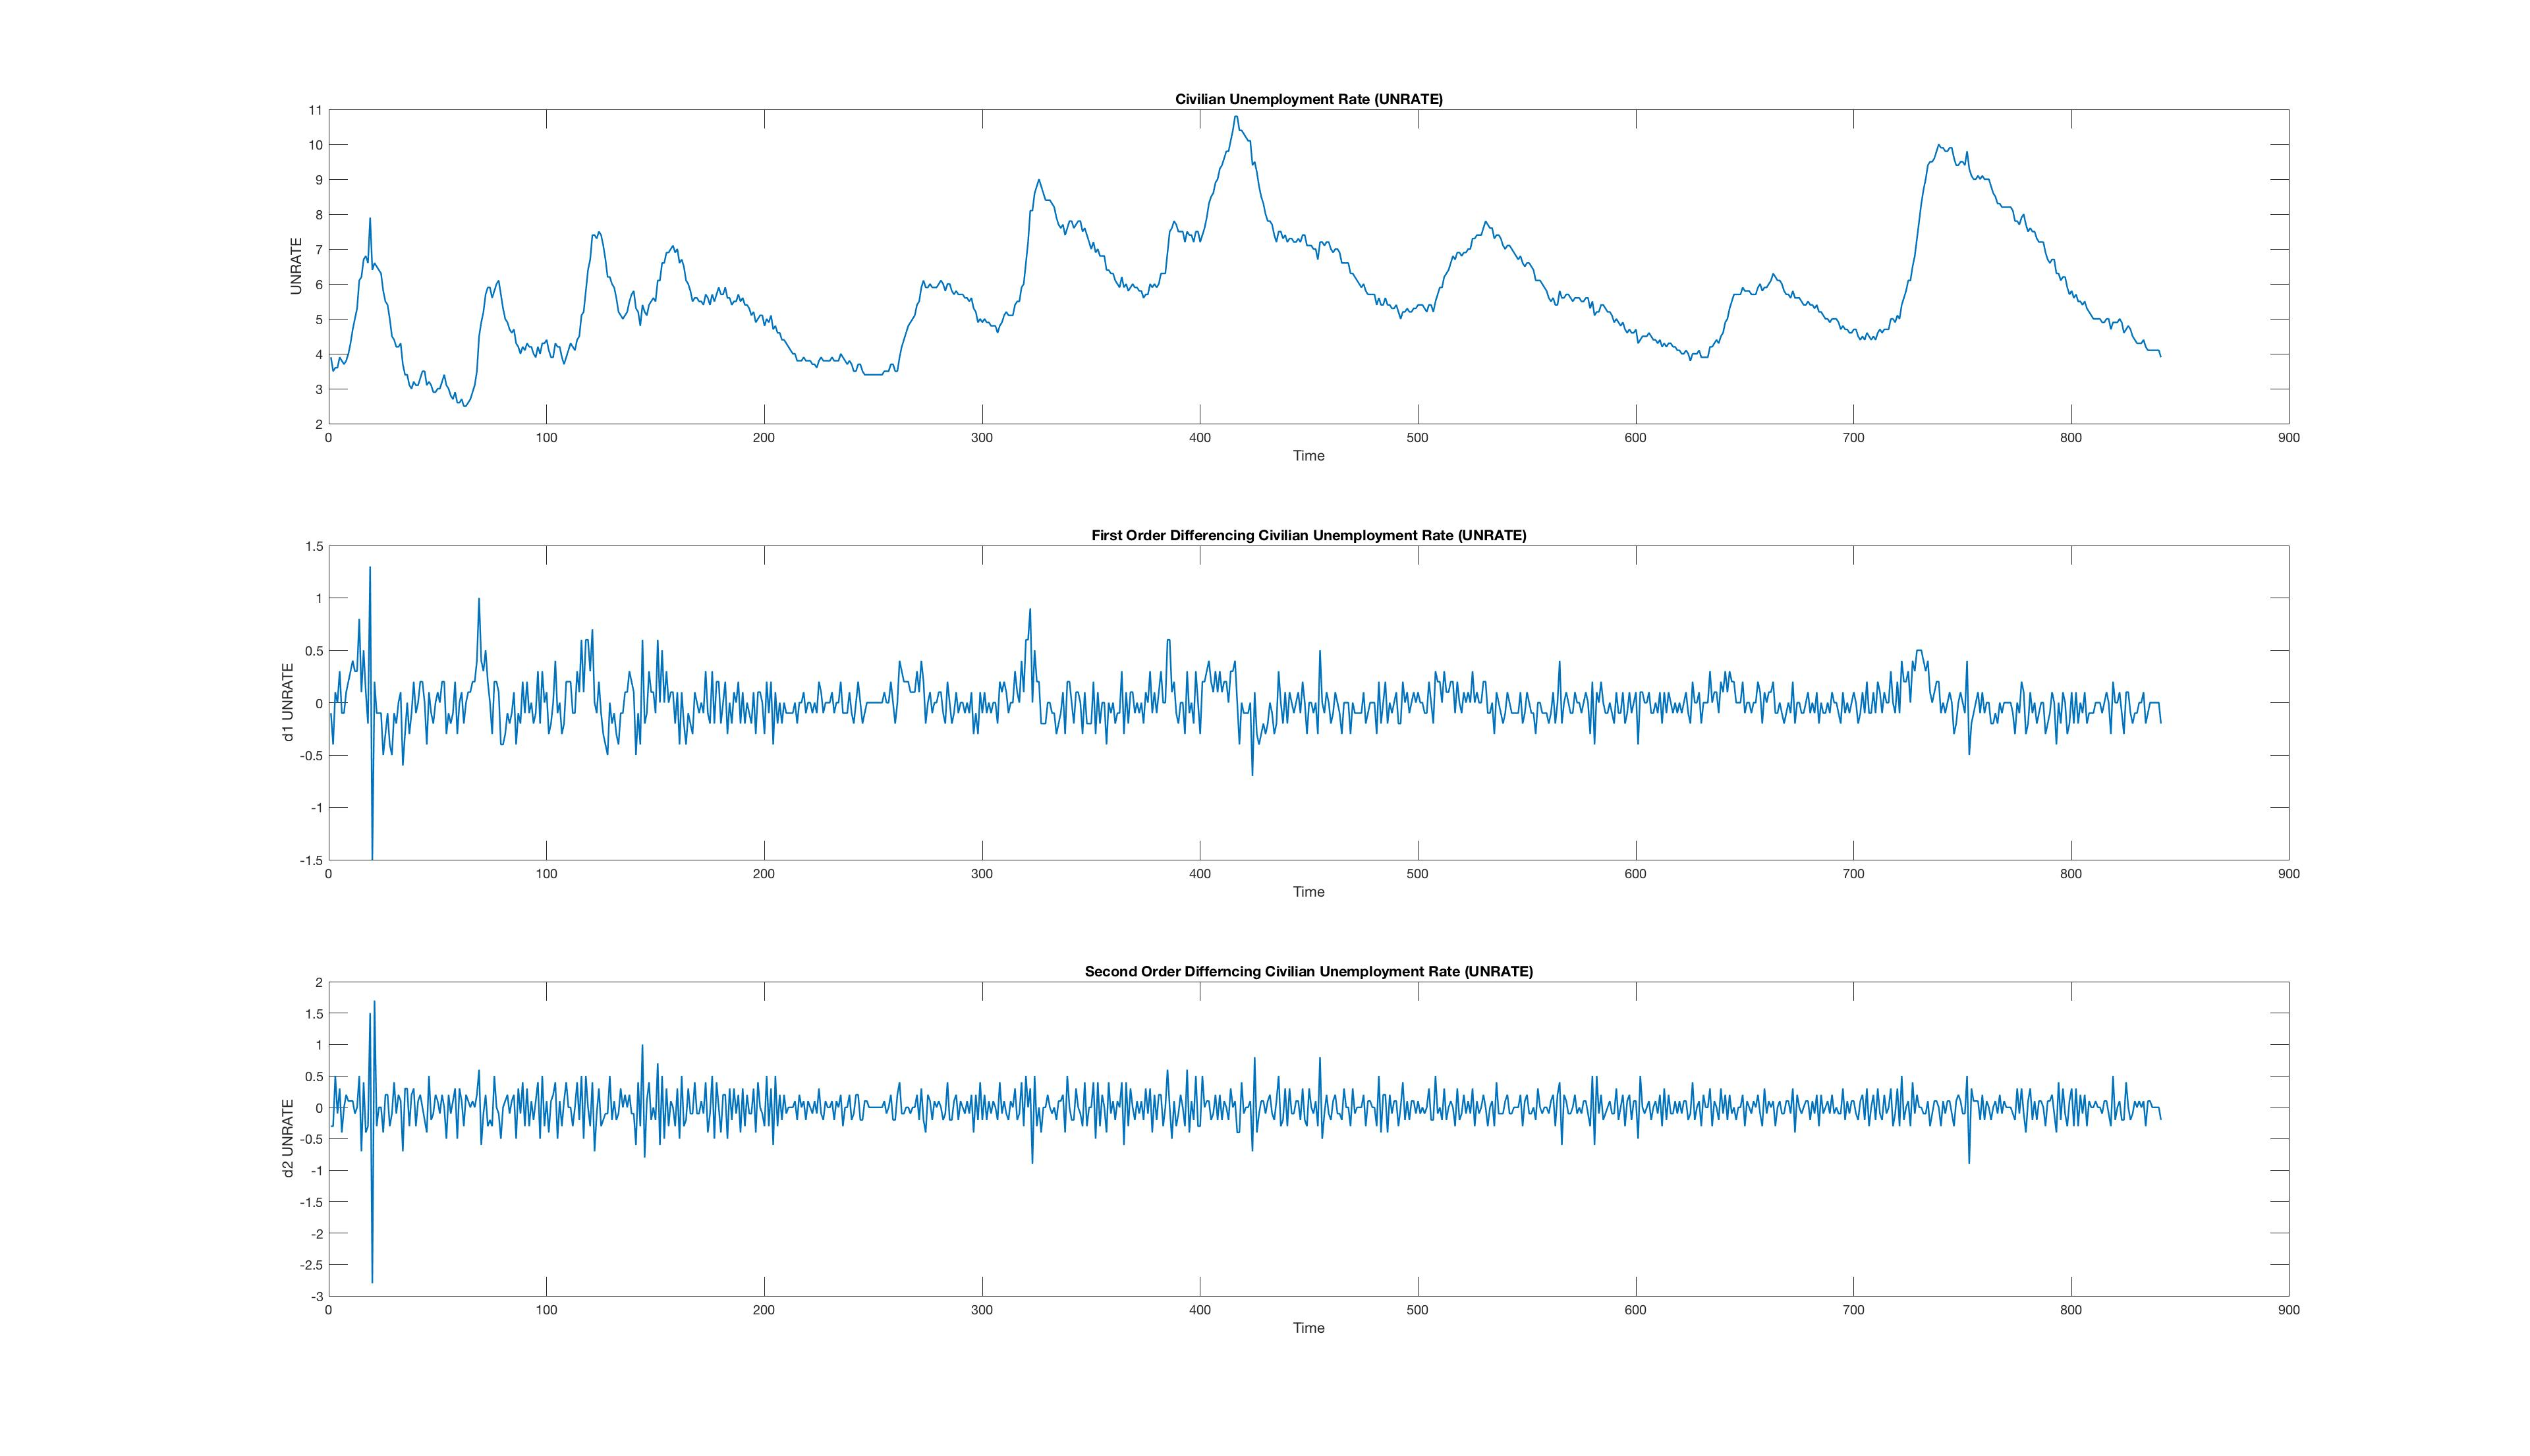
\includegraphics[width=\linewidth]{unrate_data.jpg}
    \caption{Civilian Unemployment Rate in United States}
\end{figure}

\subsection{Model architecture}
\paragraph{} Before feeding data into our model, our data are firstly mean normalized using equation (4).
\begin{equation}
    x^*_i = \frac{x_i - \overline{x}}{\sigma}
\end{equation}

The network contains six layers in total, including one input layers, two stacked Long-Short Term Memory (LSTM) layers (with sizes of 64 and 32), two stacked fully connected layers and a regression layer as the output layer. 

\section{Result}
\paragraph{} After training the model for 250 epochs, the model converges and shows a performance of $RMSE=0.0130$ on the testing set. Figure (2) plots the observed and predicted values of the unemployment rate in testing set, altogether with the RMSE values. The result of this training is stored in \texttt{essayDemo.mat} file.

\begin{figure}[H]
    \centering
    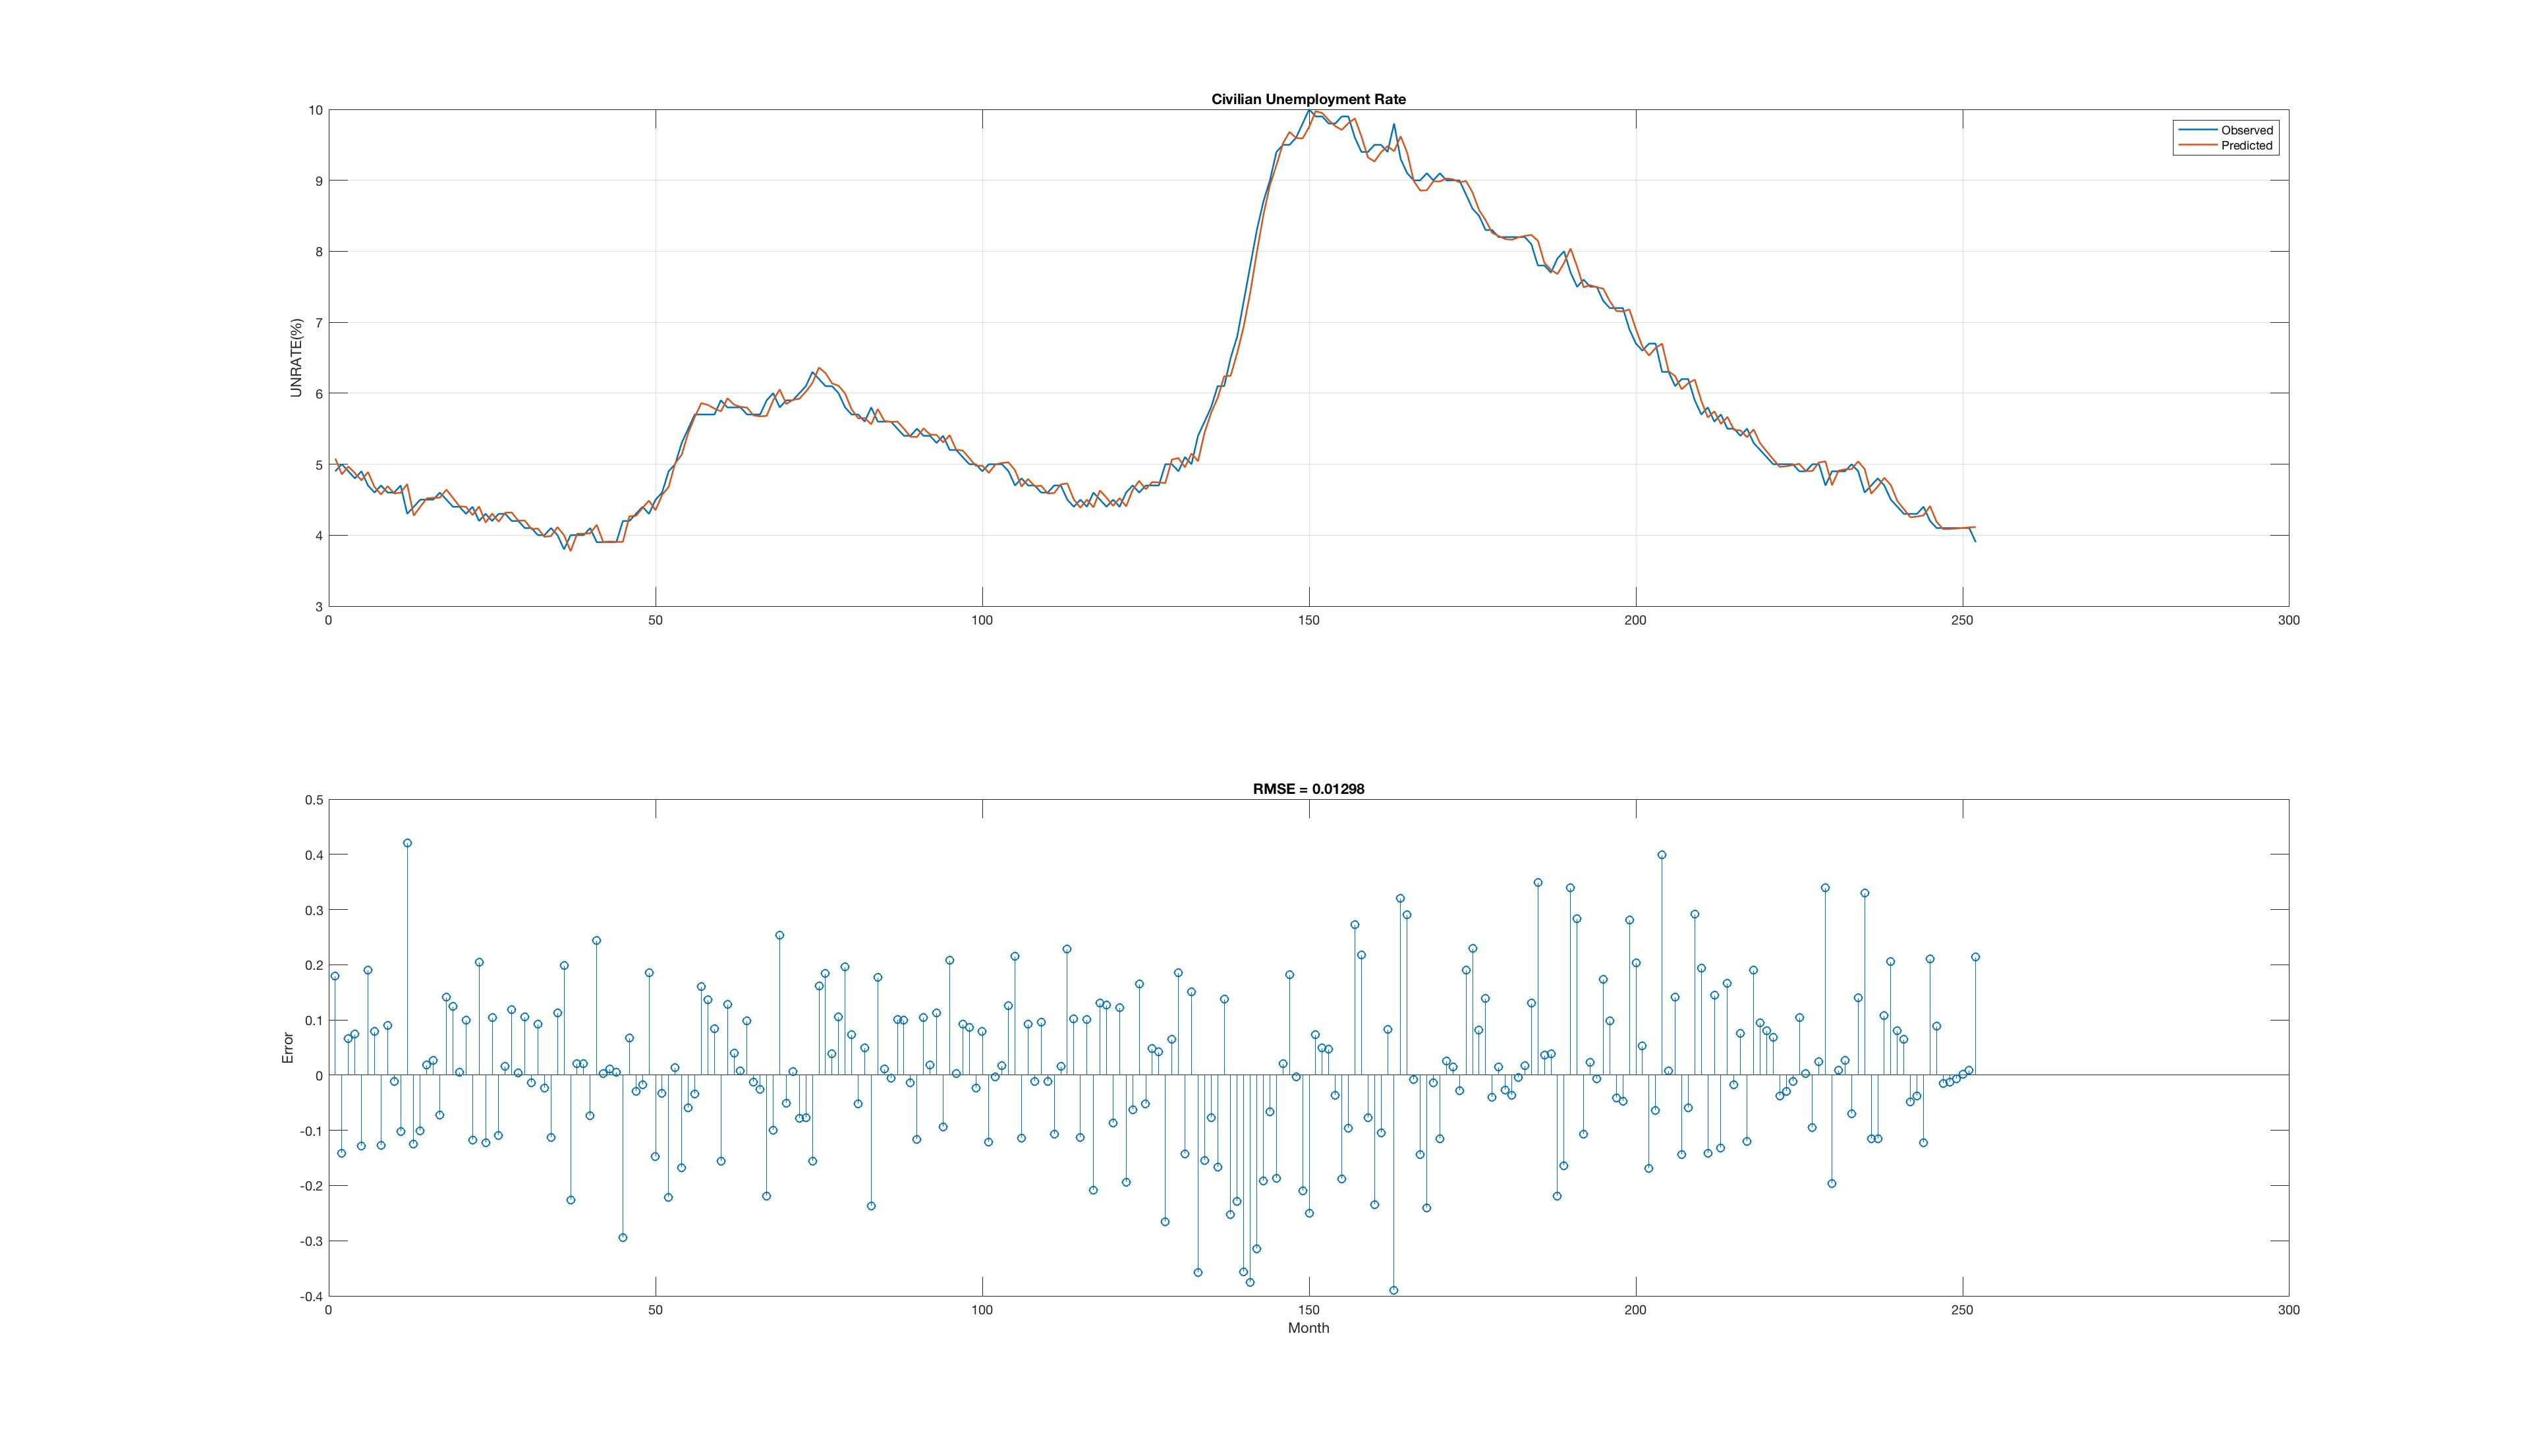
\includegraphics[width=\linewidth]{result}
    \caption{Observed value and prediction from model, after 250 epochs of training}
\end{figure}


\section{Extension: Adding Context Series into Model}
\section{Conclusion}
\section{Reference}
\end{document}
